% =========================================================================== %

\begin{frame}[t,plain]
\titlepage
\end{frame}

% =========================================================================== %

\begin{frame}{Über OpenGL und GLUT}
%
\begin{columns}[T]
\column{.5\linewidth}
\begin{itemize}
\item Multiplattform-API (\emph{Application Programming Interface} für 2D- und 3D-Anwendungen
\item Quelloffen und frei
\item Entwickelt in Zusammenarbeit mit Grafikkarten-Herstellern
\item Entwicklung seit 1992, ständige Weiterentwicklung
\item Intern in C geschrieben
\item Ca. 250 Befehle
\end{itemize}
%
\column{.5\linewidth}
\vspace{-5pt}
\href{https://www.opengl.org/}{
\includegraphics[width=\linewidth]{./gfx/OpenGL-Logo}}
\begin{itemize}
\item GLUT (\emph{OpenGL Utility Toolkit}) -- auf OpenGL basierende Routinen
\item Fenster- und Eventmanagement, Grafiken
\end{itemize}
\end{columns}
%
\vspace{15pt}
{\scriptsize Gutes Tutorial: \url{http://www.lighthouse3d.com/tutorials/glut-tutorial/}}
%
\end{frame}

% =========================================================================== %\\

\begin{frame}{Dependencies und Compileraufruf}
%
\begin{itemize}
\item openGL und GLUT
\item Windows
	\begin{itemize}
	\item \url{https://medium.com/@bhargav.chippada/how-to-setup-opengl-on-mingw-w64-in-windows-10-64-bits-b77f350cea7e}
	\item \url{http://freeglut.sourceforge.net/}
	\end{itemize}
\item Linux Debian/Ubuntu
	\begin{itemize}
	\item Einfacher Kommandozeilen-Befehl
	\item \texttt{sudo apt-get install freeglut3 freeglut3-dev}
	\end{itemize}
\item Mac
	\begin{itemize}
	\item I have no effin clue.
	\end{itemize}
\end{itemize}
%
\begin{cmdbox}[Compiler-Aufruf]
\scriptsize
gcc -std=c11 -Wall -Wextra -Wpedantic myCode.c {\color{cyan} -lglut -lGL} -o myExecutable
\end{cmdbox}
%
\end{frame}

% =========================================================================== %

\begin{frame}[fragile, t]
%
\tcbset{width=.495\linewidth, on line}
%
\begin{codebox}[Beispiel von \href{http://www.lighthouse3d.com/tutorials/glut-tutorial/}{\texttt{Lighthouse3D}} ...]
\begin{minted}[fontsize=\scriptsize, linenos]{c}
#ifdef __APPLE__
#include <GLUT/glut.h>
#else
#include <GL/glut.h>
#endif

void renderScene(void) {
   glClear(
      GL_COLOR_BUFFER_BIT | 
      GL_DEPTH_BUFFER_BIT
   );

   glBegin(GL_TRIANGLES);
      glVertex3f(-0.5, -0.5, 0.0);
      glVertex3f( 0.5,  0.0, 0.0);
      glVertex3f( 0.0,  0.5, 0.0);
   glEnd();

   glutSwapBuffers();
}
\end{minted}
\end{codebox}
%
\begin{codebox}[... ein Dreieck.]
\begin{minted}[fontsize=\scriptsize, linenos, firstnumber=last]{c}
int main(int argc, char **argv) {
   // init GLUT and create Window
   glutInit(&argc, argv);
   glutInitDisplayMode(
      GLUT_DEPTH  | 
      GLUT_DOUBLE | 
      GLUT_RGBA
   );
   glutInitWindowPosition(100, 100);
   glutInitWindowSize    (320, 320);
   glutCreateWindow("GLUT Tutorial");

   // register callbacks
   glutDisplayFunc(renderScene);

   // enter GLUT event processing cycle
   glutMainLoop();

   return 1;
}
\end{minted}
\end{codebox}
%
\end{frame}

% =========================================================================== %

\begin{frame}{GLUT -- Zentrale Konzepte}
%
\begin{columns}[T]
\column{.5\linewidth}
\begin{itemize}
\item Von GTK bekannt:
	\begin{itemize}
	\item Kontroll-Übergabe an Main-Loop in \texttt{glutMainLoop();} \vspace{3pt}
	\item Callback-Functions: von \texttt{glutMainLoop()} aufgerufen bei Events \vspace{3pt}
	\item Objekt erstellen, Eigenschaften festlegen \newline
		(\texttt{glutCreateWindow}, \texttt{glutInitWindowSize}, \texttt{glutInitWindowPosition})
	\end{itemize}
\end{itemize}
%
\column{.5\linewidth}
\begin{itemize}
\item Neue Ideen
	\begin{itemize}
	\item Wirkung auf \enquote{aktives Objekt}\newline
		(Keine Übergabe von Parameter: Welches Fenster) \vspace{3pt}
	\item Darstellungs-Modus (\texttt{glutInitDisplayMode}) \vspace{3pt}
	\item Drahtgitter-Modelle \vspace{3pt}
	\item Perspektiven und Kamera-Modelle
	\end{itemize}
\end{itemize}
\end{columns}
%
\end{frame}

% =========================================================================== %

\begin{frame}{Darstellungsmodi}
%
\begin{itemize}
\item \emph{Bitmaske} als Parameter von \texttt{glutInitDisplayMode}
	\begin{itemize}
	\item \texttt{Symbol1 = 00010$_{binär}$}
	\item \texttt{Symbol2 = 00001$_{binär}$}
	\item \texttt{Symbol1 | Symbol2  = 00011$_{binär}$}
	\item Jedes Bit aktiviert bestimmte Eigenschaften
	\end{itemize}
\item \texttt{GLUT\_DEPTH} -- 3D-Clipping -- Bestimme, was \enquote{hintereinander} steht
\item \texttt{GLUT\_RGBA} -- \emph{True-Colour-Modus}
	\begin{itemize}
	\item Jeder Pixel enthält 4 Farb-Informationen
	\item Rot-, Grün, Blau-Anteil, Transparenz
	\item Gegenstück: \emph{Palette-Indiziert} (GLUT\_INDEX) -- 1 steht für rot, 2 für gelb, ...
	\end{itemize}
\end{itemize}
%
\vspace{10pt}
{\scriptsize \url{https://www.opengl.org/resources/libraries/glut/spec3/node12.html}}
%
\end{frame}

% =========================================================================== %

\begin{frame}{Darstellungsmodi -- Single vs. Double Buffering}
%
\begin{columns}[T]
\column{.5\linewidth}
\begin{itemize}
\item \texttt{GLUT\_DOUBLE} -- Double Buffering
	\begin{itemize}
	\item Ein Arbeits-Bildschirm auf dem Bild vorbereitet wird
	\item Ein Anzeige-Bildschrim, tatsächlich sichtbar
	\item Fertige Bilder werden auf Anzeige-Bildschirm kopiert
	\item Verhindert Flackern bei Animationen
	\end{itemize}
\item Siehe \href{http://openglbook.com/chapter-1-getting-started.html}{\emph{The OpenGL Book, Chapter 1}}
\end{itemize}
%
\column{.5\linewidth}
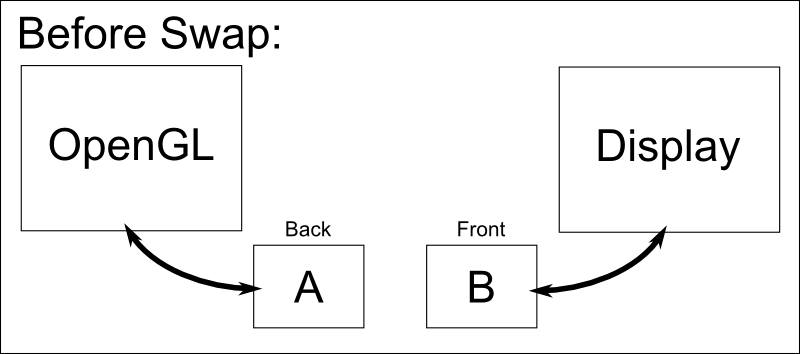
\includegraphics[width=\linewidth]{./gfx/GL-DoubleBuffer-1}\newline
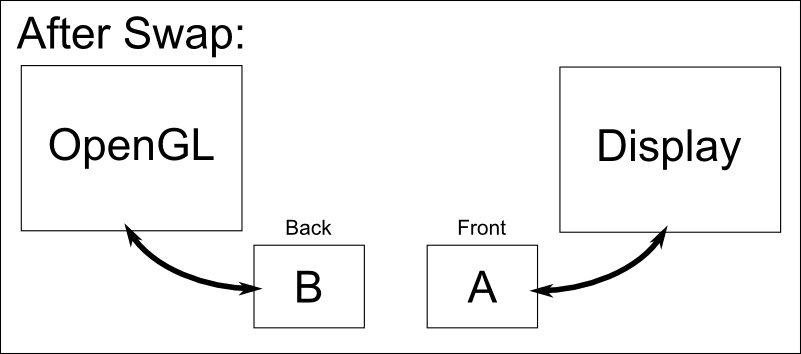
\includegraphics[width=\linewidth]{./gfx/GL-DoubleBuffer-2}
\end{columns}
%
\end{frame}

% =========================================================================== %

\begin{frame}[fragile, t]
%
\tcbset{width=.495\linewidth, on line, height=7.0cm}
%
\begin{codebox}[Kontrollfluss in main, box align=top]
\begin{tikzpicture}[
  comp/.style={shape=rectangle,draw=black,rounded corners=2pt, font=\footnotesize},
  proc/.style={shape=ellipse,draw=black, font=\scriptsize},
  flow/.style={draw=black,->,shorten >=2pt}
]
	\node at (0  , 7  ) [comp] (init) {OpenGL und glut starten};
		\node (initFrom) [left of = init, below = -1mm of init] {};
	\node at (1.5, 6.3) [proc] (gluInit) {\texttt{glutInit}};
	\draw[flow] (initFrom) |- (gluInit.west);
	
	\node at (0  , 5.5) [comp] (hWin) {Grafikfenster vorbereiten};
		\node (hWinFrom) [left of = hWin, below = -1mm of hWin] {};
	\node at (1.5, 4.1) [proc] (gluWin) {\parbox{2.7cm}
		{\texttt{glutInitDisplayMode}\\
		 \texttt{glutInitWindowPosition}\\
		 \texttt{glutInitWindowSize}\\
		 \texttt{glutCreateWindow}
		}};
	\draw[flow] (hWinFrom) |- (gluWin.west);
	
	\node at (0  , 2.6) [comp] (call) {Callbacks registrieren};
		\node (callFrom) [left of = call, below = -1mm of call] {};
	\node at (1.5, 1.9) [proc] (gluCall) {\texttt{glutDisplayFunc}};
	\draw[flow] (callFrom) |- (gluCall.west);
\end{tikzpicture}
\end{codebox}
%
\begin{codebox}[Lighthouse3D-Tutorial: main, box align=top]
\begin{minted}[fontsize=\scriptsize, linenos]{c}
int main(int argc, char **argv) {
   glutInit(&argc, argv);

   glutInitDisplayMode(
      GLUT_DEPTH  | 
      GLUT_DOUBLE | 
      GLUT_RGBA
   );
   glutInitWindowPosition(100,100);
   glutInitWindowSize(320,320);
   glutCreateWindow("GLUT Tutorial");

   glutDisplayFunc(renderScene);

   glutMainLoop();

   return 1;
}
\end{minted}
\end{codebox}
%
\end{frame}

% =========================================================================== %

\begin{frame}[fragile]{Rendering -- Das eigentliche Zeichnen}
%
\begin{columns}[T]
\column{.5\linewidth}
\begin{itemize}
\item Leeren Puffer vorbereiten -- \texttt{glClear}
	\begin{itemize}
	\item Bitmaske wie bei \texttt{glutInitDisplayMode}
	\item Lösche \enquote{eigentliches Bild} (\texttt{GL\_COLOR\_BUFFER\_BIT}) 
		und \enquote{Tiefeninformation} (\texttt{GL\_DEPTH\_BUFFER\_BIT})
	\end{itemize}
\item Neues Objekt anlegen -- \texttt{glBegin} und \texttt{glEnd}
	\begin{itemize}
	\item Verschiedene Objekte definiert
	\item Eckpunkte Definieren -- \texttt{glVertex3f}
	\end{itemize}
\item Bild als \enquote{fertig} markieren -- \texttt{glutSwapBuffers}
\end{itemize}
%
\column{.5\linewidth}
\begin{codebox}[Function \texttt{renderscene}]
\begin{minted}[fontsize=\scriptsize, linenos]{c}
void renderScene(void) {
   glClear(
      GL_COLOR_BUFFER_BIT | 
      GL_DEPTH_BUFFER_BIT
   );

   glBegin(GL_TRIANGLES);
      glVertex3f(-0.5, -0.5, 0.0);
      glVertex3f( 0.5,  0.0, 0.0);
      glVertex3f( 0.0,  0.5, 0.0);
   glEnd();

   glutSwapBuffers();
}
\end{minted}
\end{codebox}
\end{columns}
%
\end{frame}

% =========================================================================== %

\begin{frame}{Weitere GL-Formen}
%
\begin{columns}[T]
\column{.65\linewidth}
\begin{itemize}
\item \texttt{GL\_POINTS} -- einzelne Punkte (Pixel)
\item \texttt{GL\_LINES} -- unverbundene Linien
\item \texttt{GL\_LINE\_STRIP} -- verbundener Linienzug
\item \texttt{GL\_LINE\_LOOP} -- geschlossener Linienzug
\item \texttt{GL\_POLYGON} -- geschlossener Linienzug mit Füllung
\item \texttt{GL\_QUADS} -- Vierecke mit Füllung
\item \texttt{GL\_QUAD\_STRIP} -- verbundene Vierecke mit Füllung
\item \texttt{GL\_TRIANGLES} -- gefüllte Dreiecke
\item \texttt{GL\_TRIANGLE\_STRIP} -- verbundene gefüllte Dreiecke
\item \texttt{GL\_TRIANGLE\_FAN} -- verbundene gefüllte Dreiecke, gemeinsame Ecke
\end{itemize}
%
\column{.35\linewidth}
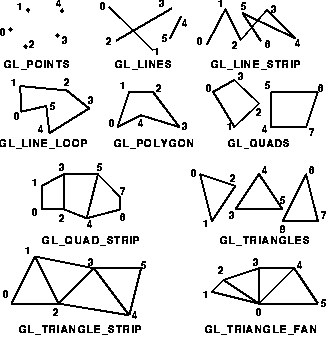
\includegraphics[width=\linewidth]{./gfx/GL-prims}\\
{\tiny\url{http://www.dgp.toronto.edu/~ah/csc418/fall_2001/tut/ogl_draw.html}}\\
\end{columns}
%
\end{frame}

% =========================================================================== %

\begin{frame}[fragile]{Farbe}
%
\begin{columns}[T]
\column{.5\linewidth}
\begin{itemize}
\item \texttt{glColor3f}
	\begin{itemize}
	\item Zuweisung einer Farbe zu einem \emph{vertex} (Eckpunkt)
	\item Auswirkung auf gesamte Fläche, falls Teil eines Flächen-Objekts
	\item Auswirkung auf Linie, falls  Teil eines Linien-Objekts
	\item Farbverläufe
	\item Farbe bleibt ausgewählt bis zum nächsten Aufruf
	\end{itemize}
\item Drei Parameter
	\begin{itemize}
	\item Rot- Grün- und Blau-Anteil der Farbe
	\item \mintinline{c}{float}-Werte zwischen 0 und 1 (Prozentwerte)
	\end{itemize}
\end{itemize}
%
\column{.5\linewidth}
\vspace{-6pt}
\begin{codebox}[Syntax: Vertex Farbe zuweisen]
\begin{minted}[fontsize=\scriptsize, linenos]{c}
glColor3f(red, green, blue);
\end{minted}
\end{codebox}
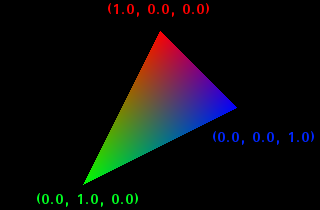
\includegraphics[width=\linewidth]{./gfx/GL-Tricolor}
\end{columns}
%
\end{frame}

% =========================================================================== %

\begin{frame}{Reshape Functions und Perspektive}
%
\begin{itemize}
\item Bei Änderung der Fenstergröße: Fensterinhalt wird mit skaliert
\item[$\Rightarrow$] Objekte werden verzerrt
\item Automatische Korrektur durch spezielle Callback-Function
\item[$\Rightarrow$] \texttt{glutReshapeFunc(changeSize);}
\item Parameter der aufgerufenen Funktion 2 \mintinline{c}{int}s für Höhe, Breite
\item Berechnung \emph{aspect ratio} (Seitenverhältnis), Übergabe an \texttt{gluPerspective}
\item Intern: Umrechnung 3D-Koordinaten in 2D-Darstellung über Matrix-Operationen
\item OpenGL stellt 2 Matrizen zur Verfügung: \emph{Model-View-Matrix} und \emph{Perspective-Matrix}
\item Verwendung ist dem Programmierer frei gestellt; empfohlen jedoch:
	\begin{itemize}
	\item \emph{Model-View-Matrix} -- Objekt bearbeiten (verschieben, drehen, etc.)
	\item \emph{Perspective-Matrix} -- Perspektive bearbeiten (\enquote{Kameraposition},
		  \enquote{Öffnungswinkel}, damit auch Seitenverhältnis Fenster).
	\end{itemize}
\end{itemize}
%
\end{frame}

% =========================================================================== %

\begin{frame}{Auswirkung der \emph{Perspective-Matrix}}
%
\begin{minipage}[l]{.46\linewidth}
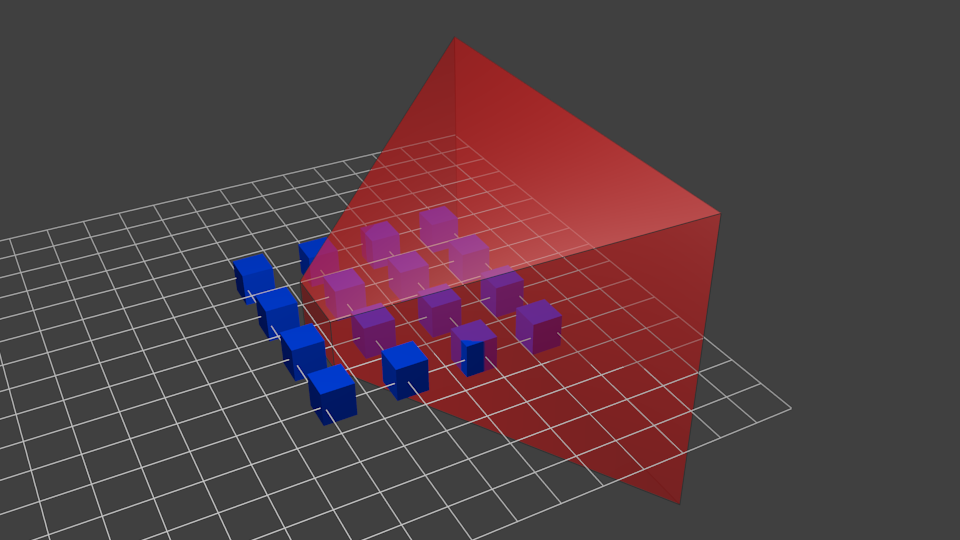
\includegraphics[width=\linewidth]{./gfx/nondeforme} 
\end{minipage}
%
\begin{minipage}[c]{.06\linewidth}
\begin{center}
$\Rightarrow$
\end{center}
\end{minipage}
%
\begin{minipage}[r]{.46\linewidth}
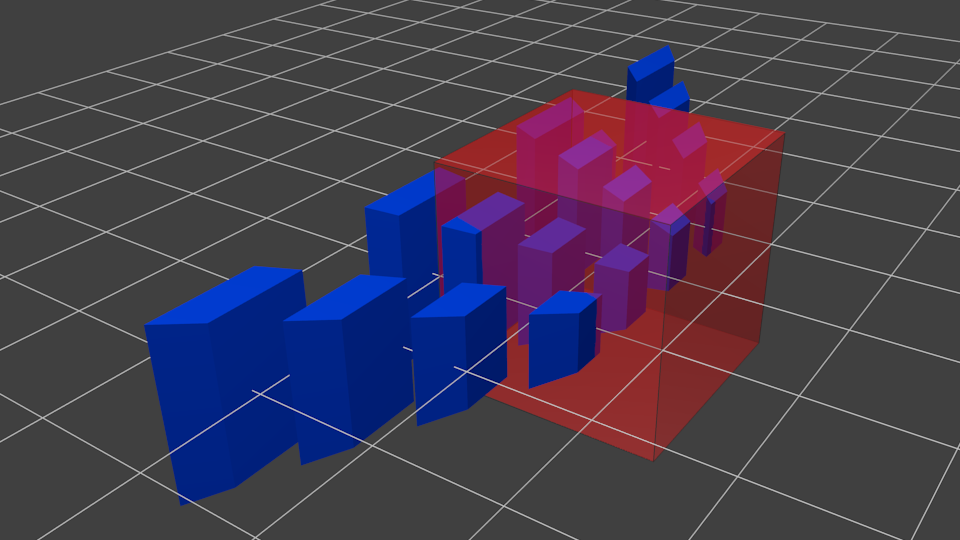
\includegraphics[width=\linewidth]{./gfx/homogeneous}
\end{minipage}
%
\begin{minipage}{.79\linewidth}
\begin{itemize}
\item Linkes Bild: Blick von links nach rechts, Sichtfeld rot
\item Rechtes Bild: Perspektivische Korrektur der Objekte -- neue Größen nach Entfernung
\item Unten: Projektion auf 2D-Fenster
\end{itemize}
{\tiny\url{http://www.opengl-tutorial.org/beginners-tutorials/tutorial-3-matrices/}}
\end{minipage}
%
\begin{minipage}{.20\linewidth}
\vspace{3pt}
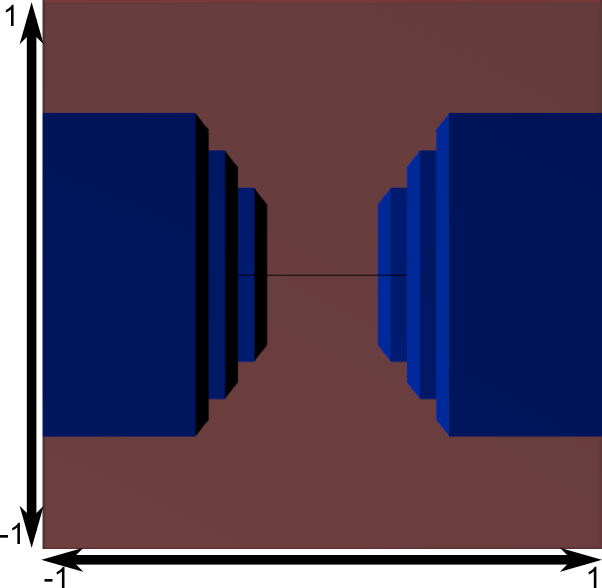
\includegraphics[width=\linewidth]{./gfx/projected1}
\end{minipage}
%
\end{frame}

% =========================================================================== %

\begin{frame}[fragile]
%
\begin{columns}[T]
\column{.5\linewidth}
\begin{Large}
{Konstruktion der Reshape-Callback}
\vspace{10pt}
\end{Large}
%
\begin{itemize}
\item Berechne Seitenverhältnis
\item \enquote{Aktiviere} Projection-Matrix
\item Starte mit 1:1-Abbildung (\texttt{glLoadIdentity})
\item Lege die Perspektive fest (\texttt{gluPerspective}). Parameter:
	\begin{itemize}
	\item Öffnungswinkel -- Blickfeld
	\item Seitenverhältnis
	\item Nah-Grenze -- Sichtbarkeit ab hier
	\item Fern-Grenze -- Sichtbarkeit bis hier
	\end{itemize}
\item Lege \emph{Viewport} fest
\item Zurück zur Modelview-Matrix
\end{itemize}
%
\column{.5\linewidth}
\begin{codebox}[Function \texttt{changeSize}, height=7.6cm]
\begin{minted}[fontsize=\scriptsize, linenos]{c}
void changeSize(int w, int h) {
   // Prevent a divide by zero
   if (h == 0) {h = 1;}
   float ratio =  (float) w / h;

   // Use the Projection Matrix
   glMatrixMode(GL_PROJECTION);

   // Reset Matrix
   glLoadIdentity();

   // Set the correct perspective.
   gluPerspective(45.0f, ratio, 1, 100);

   // Use the entire window
   glViewport(0, 0, w, h);

   // Get Back to the Modelview
   glMatrixMode(GL_MODELVIEW);
}
\end{minted}
\end{codebox}
\end{columns}
%
\end{frame}

% =========================================================================== %

\begin{frame}[fragile]{Animation}
%
\begin{columns}[T]
\column{.5\linewidth}
\begin{itemize}
\item Eigene Callback-Funktion: Leerlauf (\emph{idle})
\item \texttt{glutIdleFunc(renderScene);}
\item Eine Möglichkeit: Alle Objekte neu positionieren
\item Andere Möglichkeit: Welt als ganzes bewegen
\item[$\Rightarrow$] Änderung an \texttt{GL\_MODELVIEW}-Matrix
\item Verschieben: \texttt{glTranslatef}
\item Drehen: \texttt{glRotatef}
\item Kameraposition festlegen: \texttt{gluLookAt}
\end{itemize}
%
\column{.5\linewidth}
\begin{codebox}[gl-Bewegungen: Syntax]
\begin{minted}[fontsize=\scriptsize, linenos]{c}
glTranslatef    (x, y, z);
glRotatef(angle, x, y, z);
gluLookAt(   eyeX,    eyeY,    eyeZ,
          centerX, centerY, centerZ,
              upX,     upY,     upZ);
\end{minted}
\end{codebox}
%
{\tiny
\url{https://www.khronos.org/registry/OpenGL-Refpages/gl2.1/xhtml/glTranslate.xml}

\url{https://www.khronos.org/registry/OpenGL-Refpages/gl2.1/xhtml/glRotate.xml}

\url{https://www.khronos.org/registry/OpenGL-Refpages/gl2.1/xhtml/gluLookAt.xml}\\
}
\end{columns}

%
\end{frame}

% =========================================================================== %

\begin{frame}[fragile]
%
\begin{columns}[T]
\column{.57\linewidth}
\begin{Large}
{Usereingaben: Tastatur}
\vspace{10pt}
\end{Large}
%
\begin{itemize}
\item Zwei neue Callbacks
\item \texttt{glutKeyboardFunc(processNormalKeys);}
	\begin{itemize}
	\item \enquote{normale Taste}
	\item Alles, das ASCII-Code hat.
	\item Callback-Parameter: ASCII-Code und Mauskoordinaten während Tastaturdruck
	\end{itemize}
\item \texttt{glutSpecialFunc(processSpecialKeys);}
	\begin{itemize}
	\item \enquote{Sonder-Tasten}
	\item Pfeiltasten, Funktionstasten, ...
	\item GL-Keycode und Mauskoordinaten
	\end{itemize}
\item Abfrage von \emph{Modifiern}
	\begin{itemize}
	\item \texttt{int glutGetModifiers(void)}
	\item Gibt \emph{Bitmaske zurück}
	\end{itemize}
\end{itemize}
%
\column{.43\linewidth}
\begin{codebox}[Keyboard-Callbacks:\\ Signatur]
\begin{minted}[fontsize=\scriptsize, linenos]{c}
void processNormalKeys(
    unsigned char key, 
    int x, int y);
void processSpecialKeys(
    int key, 
    int x, int y);
\end{minted}
\end{codebox}
%
\begin{itembox}[Modifier-Bit-Symbole]
\footnotesize
	\item \texttt{GLUT\_ACTIVE\_SHIFT}
	\item \texttt{GLUT\_ACTIVE\_CTRL}
	\item \texttt{GLUT\_ACTIVE\_ALT}
\end{itembox}
{\tiny\url{https://www.opengl.org/resources/libraries/glut/spec3/node73.html}}
\end{columns}
%
\end{frame}

% =========================================================================== %

\begin{frame}[fragile]
%
\tcbset{width=.495\linewidth, on line, height=7.4cm}
%
\begin{codebox}[Lighthouse3D-Tutorial: Keyboard ...]
\begin{minted}[fontsize=\scriptsize, linenos]{c}
#include <stdlib.h>

#ifdef __APPLE__
#include <GLUT/glut.h>
#else
#include <GL/glut.h>
#endif

// globals
float red = 1, blue = 1, green = 1;
float angle = 0.0f;

void changeSize(int w, int h) {
   if (h == 0) {h = 1;}
   float ratio =  (float) w / h;
   
   glMatrixMode(GL_PROJECTION);
      glLoadIdentity();
      glViewport(0, 0, w, h);
\end{minted}
\end{codebox}
%
\begin{codebox}[... Fortsetzung]
\begin{minted}[fontsize=\scriptsize, linenos, firstnumber=last]{c}
      gluPerspective(
         45.0f, ratio, 
         0.1f, 100.0f
      );
   glMatrixMode(GL_MODELVIEW);
}

void renderScene(void) {
   glClear(
      GL_COLOR_BUFFER_BIT | 
      GL_DEPTH_BUFFER_BIT
   );
   glLoadIdentity();   // Reset matrix
   gluLookAt(          // Set the camera
         0.0f, 0.0f, 10.0f,  // cam pos
         0.0f, 0.0f,  0.0f,  // look at
         0.0f, 1.0f,  0.0f   // up dir.
   );
   glRotatef(angle, 0.0f, 1.0f, 0.0f);
\end{minted}
\end{codebox}
%
\end{frame}

% =========================================================================== %

\begin{frame}[fragile]
%
\tcbset{width=.495\linewidth, on line, height=7.0cm}
%
\begin{codebox}[Lighthouse3D-Tutorial: Keyboard ...]
\begin{minted}[fontsize=\scriptsize, linenos, firstnumber=last]{c}
   glColor3f(red,green,blue);
   glBegin(GL_TRIANGLES);
      glVertex3f(-2.0f, -2.0f, 0.0f);
      glVertex3f( 2.0f,  0.0f, 0.0f);
      glVertex3f( 0.0f,  2.0f, 0.0f);
   glEnd();

   angle+=0.1f;

   glutSwapBuffers();
}

void processNormalKeys(
   unsigned char key, 
   int x, int y
) {
   if (key == 27) {exit(0);}
}
\end{minted}
\end{codebox}
%
\begin{codebox}[Lighthouse3D-Tutorial: Keyboard ...]
\begin{minted}[fontsize=\scriptsize, linenos, firstnumber=last]{c}
void processSpecialKeys(
   int key, int x, int y
) {
   switch(key) {
      case GLUT_KEY_F1 : red   = 1.0;
                         green = 0.0;
                         blue  = 0.0; 
                         break;
      case GLUT_KEY_F2 : red   = 0.0;
                         green = 1.0;
                         blue  = 0.0; 
                         break;
      case GLUT_KEY_F3 : red   = 0.0;
                         green = 0.0;
                         blue  = 1.0; 
                         break;
   }
}
\end{minted}
\end{codebox}
%
\end{frame}

% =========================================================================== %

\begin{frame}[fragile]
%
\tcbset{width=.495\linewidth, on line, height=7.0cm}
%
\begin{codebox}[Lighthouse3D-Tutorial: Keyboard  ...]
\begin{minted}[fontsize=\scriptsize, linenos, firstnumber=last]{c}
int main(int argc, char **argv) {
   // init GLUT and create window
   glutInit(&argc, argv);
   glutInitDisplayMode(
      GLUT_DEPTH | 
      GLUT_DOUBLE | 
      GLUT_RGBA
   );
   glutInitWindowPosition(100,100);
   glutInitWindowSize    (320,320);
   glutCreateWindow(
      "Lighthouse3D- GLUT Tutorial"
   );

   // rendering callbacks
   glutDisplayFunc(renderScene);
   glutIdleFunc   (renderScene);
   glutReshapeFunc(changeSize);
\end{minted}
\end{codebox}
%
\begin{codebox}[... Fortsetzung]
\begin{minted}[fontsize=\scriptsize, linenos, firstnumber=last]{c}
   // keyboard callbacks
   glutKeyboardFunc(
      processNormalKeys
   );
   glutSpecialFunc(
      processSpecialKeys
   );

   // pass control to GLUT
   glutMainLoop();

   return 1;
}
\end{minted}
\end{codebox}
%
\end{frame}

% =========================================================================== %

% http://www.opengl-tutorial.org/beginners-tutorials/tutorial-3-matrices/
% http://openglbook.com/chapter-1-getting-started.html
% https://www.khronos.org/registry/OpenGL-Refpages/gl2.1/xhtml/glBegin.xml
% https://www.khronos.org/opengl/wiki/Main_Page